\section{Software Architecture Views}
This chapter describes what our software architecture looks like. First the subsystems are identified and explained. Then the software to hardware mapping is explained, followed by how we store persistent data. Lastly concurrency between information is explained.

\subsection{Design Principle: Separation of Concerns}
Following the design principle of Separation of Concerns for separating a computer program into distinct sections, we decided to implement the three models in such a way that they can be used as separate executables. They will be connected with each other in a pipelined manner in the main tab of the program to make them part of the workflow of the program. But these models can also be seen as standalone application: by specifying a dataset and wanted output you could also use the models outside of our program.
 
\subsection{Hardware Software Mapping}

Our program is designed for a single computer. The program also runs as one process. However, in future extensions we would like to make the program multi threaded. This would enable the user to run the optimization and visualization models in separate threads. This way the program will be able to optimize the entered flight trajectory while already visualizing the noise contours of the original (unoptimized) trajectory.
Also reading in the files could be put into a separate thread. This means that all the identifiers that are read could be shown in the select tab, the moment the thread reads them.

\subsection{Persistent data management}

For this program it is not required to store information persistently. The output of the program is stored as a KML file for visualization. The format of the output is structured in such a way that it can directly be entered into Google Earth and different visualization objects can be turned on or off in Google Earth.

The state of the program can also be stored easily by saving the intermediate results of the pipeline. For example, the output of the noise model or the optimization model can be stored as a .csv file to be read in at a later point in time. This can be stored in a user specified directory. After the file is loaded in the program, the program will be able to continue where the user left off. This also means that changes to intermediate results, that will be entered as input into the next model in the pipeline, will not require changes to the input file you used at the beginning. More on this can be found in section 2j. External Major Technologies.
 
Lastly, the possibility to store the KML files for visualization also enables the user to visualize multiple flight routes in Google Earth at the same time.

\subsection{Concurrency}
This subchapter is meant to describe how concurrency issues are solved. Because it is not possible that the program is used by multiple people at the same time and the data analysis is not divided over different processes, there are no concurrency issues. However, when multiple threads are going to be used in future projects, it becomes very important to think about concurrency. This could be useful when an ATO researcher wants to read in the next flight trajectory while the previous trajectory is still being optimized or visualized in the program. Our client let us know that this is not one of his requirements.

\newpage 

\subsection{Diagram of the architecture}

Here is a diagram of our layered architecture and the connection between the front-end and the back-end: \\

\begin{center}
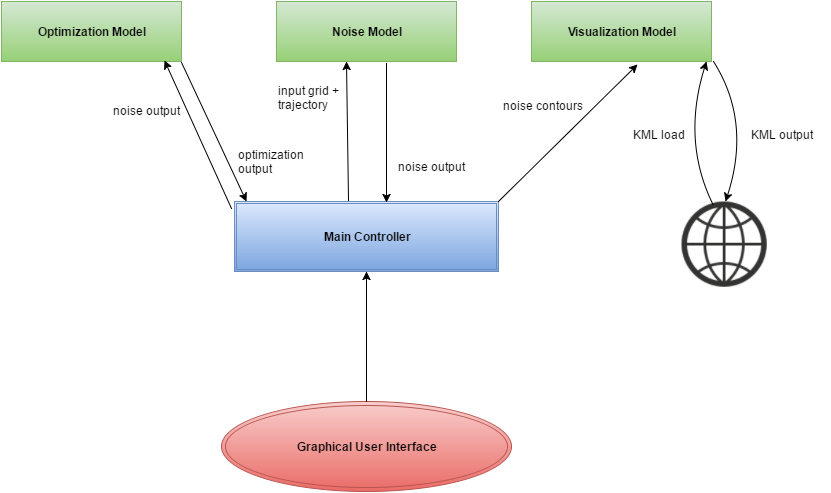
\includegraphics[width= 0.65\textwidth]{images/EmergentArchitecture} \\
\end{center}

As depicted in the diagram above, the models present the subsystems described in the Subsystem Decomposition section of the first chapter. They will exchange their outputs with the main presenter which uses the output of one system as input for the next one. The main presenter relegates the output of the the noise model to the visualization model. Based on the actual noise values the visualization model constructs the noise contours. The noise contours will be transformed into KML files and entered into Google Earth for visualization. Changes to the KML files will automatically be transferred to Google Earth by a 'KML load' script, which periodically loads the files into Google Earth.

The noise contours will also be outputted tho the main presenter. The main presenter then hands the noise contours together with the current trajectory to the optimization model. The optimization model updates the trajectory to reduce the produced noise and passes the updated trajectory on to the main controller. Now the workflow of the program can start all over again by the main presenter entering the updated trajectory into the noise model.

Following this method the models are executed in a pipelined manner. But given the right input files, the subsystems can also be run separately from each other and function as standalone applications.

%The diagram also shows the connection between the frond-end and back-end of the system. Each subsystem contains an import component that collaborates with an import controller which controls the view of the noise, optimization and visualization tabs in the GUI. This is where the user specifies which data files he or she wants to import. 
